\chapter{数据迁移框架设计}
GlusterFS\cite{GlusterFS}是一个开源、扩展能力强大的分布式文件系统,其客户端与存储服务器可通过InfiniBand RDMA或者TCP/IP等多种方式连接,并使用统一的命名空间管理数据,可将不同类型的存储服务器整合在同一个命名空间中,从而为各种工作负载和应用场景提供出色的性能。 GlusterFS服务器兼容POSIX标准,支持诸如ext4、XFS等扩展属性文件系统,可以使用包括(Network File System)和SMB(Server Message BLock)等在内的业界标准访问协议进行访问。GlusterFS专为当前高性能虚拟化云环境而设计,也可用于在并行文件系统之上搭建大规模科学与工程计算文件系统。 

本章的主要内容是在GlusterFS架构的基础上,以上一章介绍的文件分类模型为核心部件设计的智能分层存储管理框架。

\section{整体设计}





%\begin{itemize}
%    \item 全局命名空间。
%    \item 集群存储管理。
%    \item 模块化的层次机构。
%    \item 内置replication and geo-replication特性。
%    \item 自修复功能。
%    \item 高效负载均衡。
%\end{itemize}
\begin{figure}[htp]
\centering
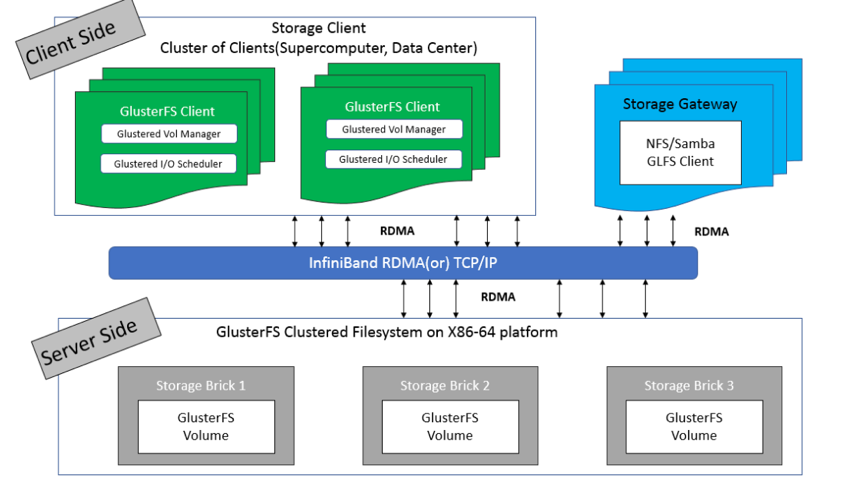
\includegraphics[width=\textwidth]{GlusterFS_Arc}
\caption{GlusterFS整体架构图}
\label{fig:GlusterFS_Arc}
\end{figure}
如图\ref{fig:GlusterFS_Arc}所示,GlusterFS服务端以存储块(Storage Brick)为硬件存储单元,可挂载于磁盘、固态硬盘、内存等多种存储介质。逻辑卷(Volume)是文件系统中的逻辑存储单元,每一个逻辑卷可由一个或者多个存储块构成,绝大多数gluster管理操作是在卷上进行的。GlusterFS根据用户需求能够支持多种逻辑卷,主要包括:

分布式卷(Distributed Volume):文件通过hash算法将数据分布到所有存储服务器上,这种卷是glusterfs的基础和最大特点;其本质功能是扩大的磁盘空间,如果有一个磁盘损坏,其数据也丢失,文件级RAID 0,不具有容错能力。

复制卷(Replicated Volume):此类逻辑卷将文件同步复制到多个brick上,文件级RAID 1,具有容错能力,同等硬件条件下写性能下降,但读性能有所提升。

条带卷(Stripe Volume):类似RAID0,文件分成数据块以Round Robin方式分布到存储服务器上,并发粒度是数据块,支持超大文件,大文件的读写性能优异。

复合卷:所谓复合卷主要包括分布式条带卷、分布式复制卷、条带复制卷和分布式条带复制卷等,兼具了基本卷的优点,在实际应用场景下较常见。



%\subsection{层叠式模块化设计}
\begin{figure}[htp]
\centering
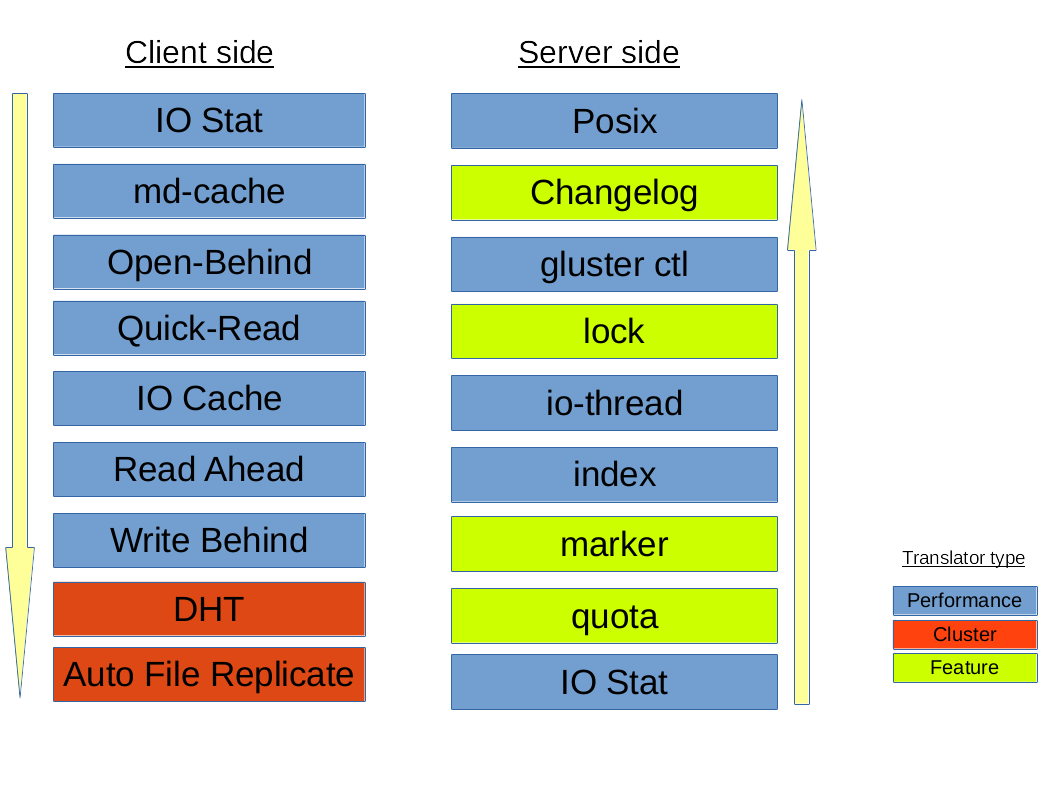
\includegraphics[width=\textwidth]{translators}
\caption{由模块(Translators)堆叠组成的堆栈式结构}
\label{fig:translators}
\end{figure}
Translator是GlusterFS中处理文件请求,实现各类文件操作功能的模块
\cite{BWFS}\cite{DPFS}。
如图\ref{fig:translators}所示,不同功能的模块以动态链接库的方式加载,以函数调用的形式逐级传递和处理文件操作请求,并通过回调函数传回文件操作结果或读取的数据。客户端和服务端之间的消息传递则通过远程过程调用(Remote Procedure Call)实现。
Translator模块是GlusterFS实现诸多功能的主要组件,每一层translator模块内均可对POSIX文件操作函数(打开文件、读写数据和元数据访问等)重新定义,可通过修改参数或修改回调数据等方式实现特定功能。Translator模块以一对一或一对多的方式堆叠组合实现更复杂的功能。

%GlusterFS主要包括cluster,performance,features,protocal,storage,encryption等几类模块。其中cluster类模块是实现存储集群功能的核心,包括分布式哈希表(DHT),
GlusterFS主要包括以下几组translator模块:

集群模块组(Cluster Translators)。主要包括分布式哈希表(DHT)、自动文件备份(AFR)等模块,是构成存储服务器集群功能的核心组件。GlusterFS没有采用元数据服务器定位文件数据,而是采用弹性哈希算法定位文件,首先根据文件路径计算哈希值,然后根据哈希值定位到具体的brick存储单元进行文件定位。AFR模块的功能则是自动冗余备份(为避免分歧,通常备份数据多于两个),当发生数据丢失或损坏时进行数据修复。

性能模块组(Performance Translators)。此类模块的目的是对GlusterFS的整体性能进行优化,如io-cache在GlusterFS进程的内存池内空闲部分开辟空间用于缓存;io-threads用于多线程管理;md-cache用于元数据缓存服务;read-ahead用于预读数据;write-back实现写回功能提升写数据性能等等。

功能模块组(Feature Translators)。主要包括日志管理模块changelog,全局锁管理locks模块等等。

协议模块组(Protocol Translators)。GlusterFS架构下,客户端与存储服务端互联方式多种多样,通过协议模块组实现对多种标准协议的支持。

存储模块组(Storage Translators)。实现GlusterFS与本地POSIX文件系统的接口。

加密模块组(Encryption Translators)。顾名思义,可以在此类模块中灵活定义不同的加密算法以保证数据安全性。

调试模块组(Debug Translators)。

Tiering模块是GlusterFS自3.7版本之后开始支持的分层数据管理模块\cite{Tiering}。与传统分层存储思想类似,文件数据被冠以“热”与“冷”的分类标签,即,访问频繁的文件为“热”数据,反之为“冷”数据。在Tiering模块的实现中,同一逻辑卷被同时挂载到“冷热”两类brick存储单元,“热”存储单元(通常为高性能存储介质如DRAM或SSD等)被视为“冷”存储(廉价、性能较弱的磁盘)的上一级缓存,因此文件的“冷热”对用户应用透明,完全由tiring模块负责文件分类与缓存调度。

\begin{figure}[htp]
\centering
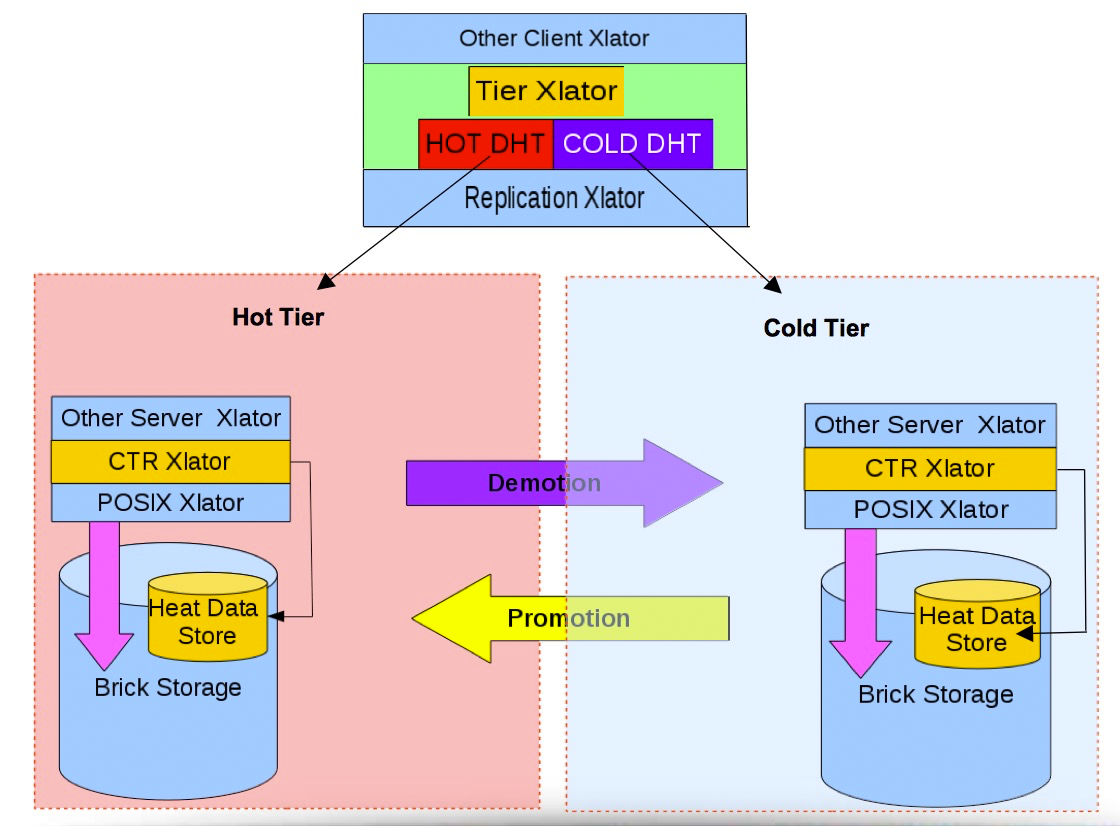
\includegraphics[width=\textwidth]{tiering}
\caption{Tiering模块原理}
\label{fig:tiering}
\end{figure}

如图\ref{fig:tiering},当GlusterFS启用tiering模块时,原本的分布式哈希算法模块被调整为“热”哈希模块与“冷”哈希模块。文件定位与查找优先在“热”存储内进行,若查找成功就是一次缓存命中;反之发生缓存缺失时通过“冷”哈希模块将请求转发到“冷”存储进行重新定位查找。

传统缓存替换算法LRU的实现过程中的核心指标是数据近期访问次数(通常存储于访问速度最快的L1-cache中),近期最少访问的数据被淘汰,而tiering模块则沿用了这一思想。区别在于tiering模块中缓存置换的粒度远远大于CPU cache或内存级的缓存,大多数应用场景是将SSD作为磁盘阵列的缓存,需要迁移置换的数据量大(大文件或海量小文件),同时算法的时间粒度也要宽松得多。

Tiering模块只实现了基本的LRU缓存,缓存不友好的工作负载会导致性能下降。为了使Tiering模块适应更多复杂的工作负载,优化分层存储性能,本文应用前面建立的文件分类模型提出了一套智能分层存储管理方案,整体设计如图\ref{fig:design_architecture},当系统初始化时,预训练的词向量模型和循环神经网络模型将被复制到挂载点根目录下,客户端与服务端的模块均可访问。下面对客户端和服务端的功能设计进行分别介绍。
%主要内容包括MDC模块(位于客户端)和修改后的CTR模块(服务端),以及做出相应修改的GFDB数据库和数据迁移后台程序。

\begin{figure}[htp]
\centering
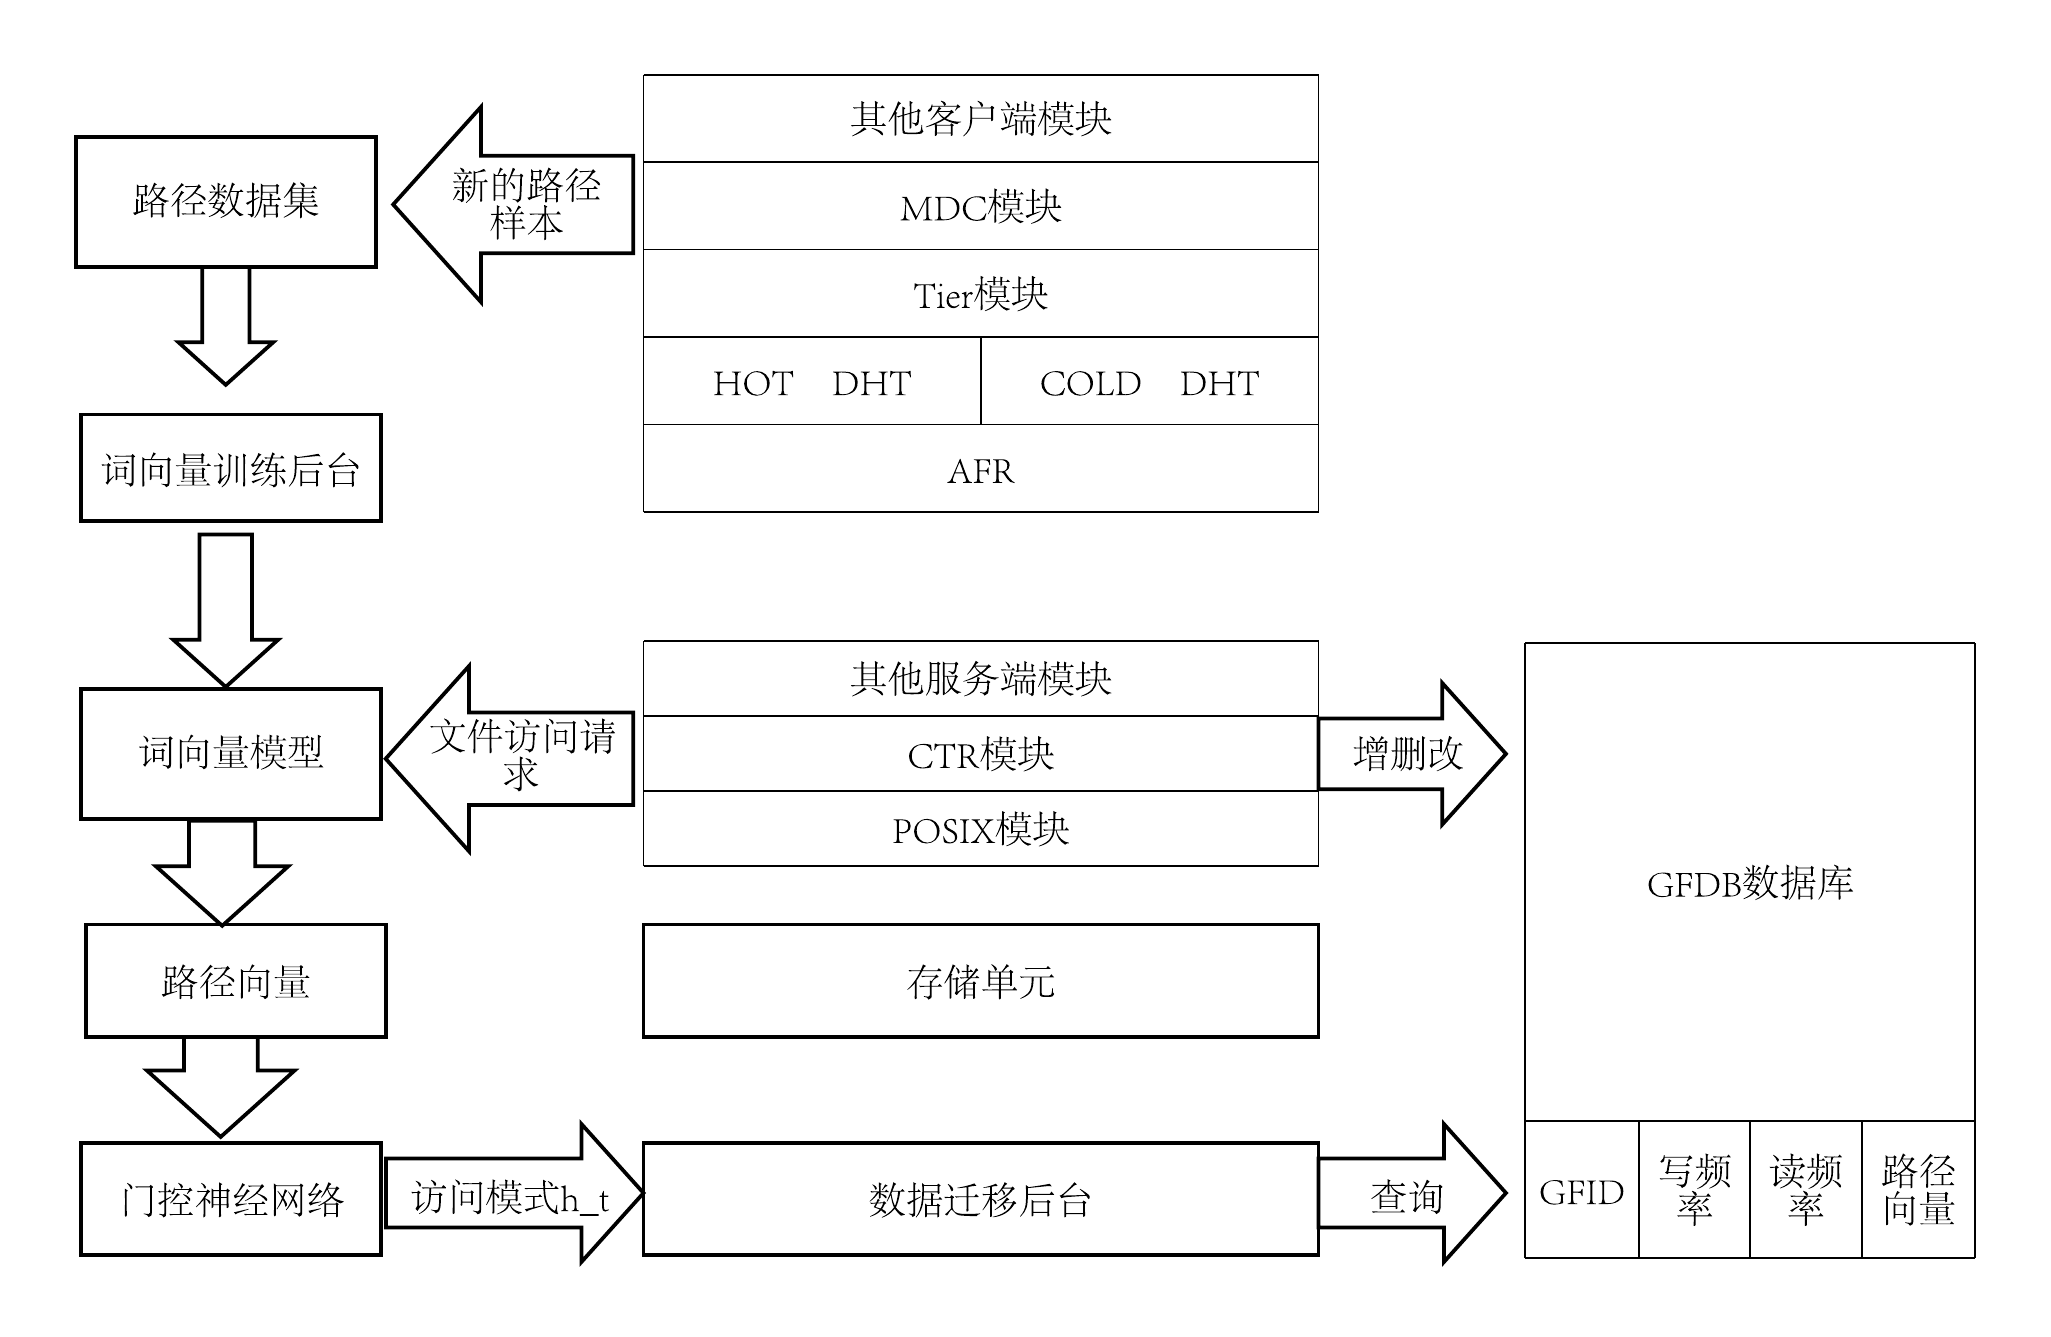
\includegraphics[width=\textwidth]{design_arch}
\caption{整体设计框图}
\label{fig:design_architecture}
\end{figure}

\section{客户端设计}


在本设计方案中,客户端添加了一个新的模块MDC(Meta Data Changelog)。该模块主要作用是监控元数据写操作以及训练词向量模型。

\begin{table}[htbp]
\centering
\begin{minipage}[t]{0.9\linewidth}
\caption{MDC模块监控的元数据写操作}
\label{tab:mdc_fops}
\begin{tabularx}{\linewidth}{cZ}
\toprule[1.5pt]
{\hei 函数名} & {\hei 功能}\\
\midrule[1pt]
create() & 创建文件 \\
mknod() & 创建文件 \\
mkdir() & 创建目录 \\
remove() & 删除 \\
rename() & 重命名 \\
link() & 创建链接 \\
symlink() & 创建符号链接 \\
unlink() & 删除链接 \\
... & ... \\
\bottomrule[1.5pt]
\end{tabularx}
\end{minipage}
\end{table}

表\ref{tab:mdc_fops}中所列函数会改变文件目录结构,当累计的改变过大,以原来目录结构训练的词向量模型可能会失效。设计MDC模块的主要目的就是随着文件系统的持续运行,对预训练的词向量模型进行迁移训练,以适应新的目录结构。基于此目的,MDC模块维护一个元数据写操作计数器mdc\_counter,每一次元数据写操作将导致该计数器按目录层级加权递增。与此同时,该操作会被作为一次“事务”写入日志文件,该日志文件用于生成新的词向量训练样本。当计数器达到阈值时,MDC模块将启动词向量训练后台线程进行迁移训练,直至模型重新收敛后结束线程并将计数器和日志清空。

\subsection{服务端设计}
GlusterFS基于sqlite3实现了一个专门用于记录文件访问记录的数据库GFDB。该数据库用于记录存储单元内所有已知文件的元数据,作为文件“冷热”分类的依据。

\begin{table}[htbp]
\centering
\begin{minipage}[t]{0.9\linewidth}
\caption{Libgfdb中的元数据结构}
\label{tab:libgfdb_file}
\begin{tabularx}{\linewidth}{cZ}
\toprule[1.5pt]
{\hei 数据项} & {\hei 描述}\\
\midrule[1pt]
GF\_ID & 文件的GFID\\
W\_SEC, W\_MSEC & 写操作请求发起(wind)时间\\
UW\_SEC, UW\_MSEC & 写操作返回(unwind)时间\\
U\_READ\_SEC, W\_READ\_MSEC & 读操作请求发起时间\\
UW\_READ\_SEC, W\_READ\_MSEC & 读操作返回时间\\
WRITE\_FREQ\_CNTR & 写操作频率\\
READ\_FREQ\_CNTR & 读操作频率\\
\bottomrule[1.5pt]
\end{tabularx}
\end{minipage}
\end{table}

\begin{table}[htbp]
\centering
\begin{minipage}[t]{0.9\linewidth}
\caption{Libgfdb目录项(Directory Entries)}
\label{tab:libgfdb_flink}
\begin{tabularx}{\linewidth}{cZ}
\toprule[1.5pt]
数据项 & 描述\\
\midrule[1pt]
GF\_ID & 文件的GFID(复合主键)\\
GF\_PID & 父目录的GFID(复合主键)\\
FNAME & 文件名(复合主键)\\
FPATH & 完整路径\\
W\_DEL\_FLAG & 文件删除(unlinked)标志\\
LINK\_UPDATE & 文件重命名标志\\
\bottomrule[1.5pt]
\end{tabularx}
\end{minipage}
\end{table}

表\ref{tab:libgfdb_file}记录了所有已知文件的访问情况,包括文件操作的起始时间,访问频率等。表\ref{tab:libgfdb_flink}本质上是GFDB维护的目录入口表,主要用于文件查找。

%服务端的设计围绕训练好的门控神经网络展开,主要工作包括GFDB数据库内容的调整,CTR模块的修改,最终目的是为复杂工作负载下的数据迁移提供决策支持。






如表格\ref{tab:libgfdb_file}所述,GFDB存储的文件元数据包括读写操作的发起时间,结束时间及最近访问频率,主要为LRU缓存策略服务。为了应用本文提出的文件分类模型,为该数据库添加了新的元数据项:文件向量,作为后续数据迁移策略的参数之一。文件向量由客户端MDC模块训练好的词向量模型计算得到。

服务端实现分层存储管理功能的关键模块是访问计数器模块CTR(Change Time Recorder)。该模块位于底层POSIX模块之上,其主要功能是对存储单元内所有文件的访问情况进行记录,包括近期内数据读、数据写和元数据写等操作的执行次数等,用于更新GFDB数据库。

当一个逻辑卷启用tiering模块时,将会在后台开启数据迁移进程。该进程周期性地查询数据库,以获得最近的文件访问情况,从而完成迁入(promotion)与迁出(demotion)的数据迁移操作。

%在系统运行过程中,数据迁移决策受到热存储占用率的影响。默认设置下,当热存储占用未达到75\%时,即便没有达到周期性迁移的时间节点,系统也会自动将冷存储单元内的高频率访问文件迁入热存储单元,以防止迁出过多数据导致缓存空间的浪费;当热存储占用超过默认的90\%时,将自动地触发迁出操作,以防止到达缓存容量上限降低整体性能。

GlusterFS实现的tiering模块主要采用传统的LRU算法设计,能够显著改善大文件的连续读操作,但对于一些不具备“缓存友好”性质的工作负载,例如多客户端并发访问大量小文件的场景下,tiering的性能反而会严重下降
\cite{Red_Hat_Gluster_storage_on_supermicro_storage_servers_powered_by_Intel_Xeon_processors}。
其本质原因是随着小文件数量大幅增加,且多客户端的并发文件请求数量上升时,传统缓存置换算法考虑的时间局部性和空间局部性失去效用,仅仅简单地以文件访问频率作为考量不足以分析提取复杂场景下的I/O访问模式。由于缓存命中率过低,而数据迁移线程运行时误判频繁,导致过多不必要的数据迁移降低了性能;另一方面,数据库访问带来的开销却不会因此而减少。

为了解决上述问题,在适当的条件下采用文件分类模型代替LRU缓存算法,本设计对CTR模块进行了改进,除了统计文件访问、更新数据库之外,该模块被赋予了新的功能:在内存中保存$N$条访问请求,当缓存命中率下降到某个阈值时,启动热点数据识别线程(即训练好的门控神经网络),并将最近保存的$N$条访问请求转化为路径向量序列作为输入,计算门控神经网络当前时刻的隐状态$\mathbf{h}_t$并发送给数据迁移线程。

此时数据迁移线程暂停执行LRU策略,即不再查询文件的访问频率,而是从数据库中批量导出n条文件的路径向量组成$n\times d$的矩阵$M$,计算模型输出层:
\begin{equation}
    \mathbf{y}_t = \sigma(M \times \mathbf{h}_t)
\end{equation}
其中$\mathbf{y}_t$各个分量表示的是对应文件判为热点数据的概率,最后根据判定阈值$0<\alpha<1$给出策略:如果该数据库隶属于热存储单元,所有概率值低于$\alpha$的文件被标记为冷数据,迁出到冷存储单元;如果该数据库隶属于冷存储单元,所有概率值高于$\beta$的文件被标记为热数据,迁入到热存储单元。









\section{本章小结}
本章介绍了分布式文件系统GLusterFS的整体架构,并详细阐述分析了Tiering模块的设计原理和不足之处,即该模块的分层存储管理停留于最基本的LRU算法,在面对缓存不友好的工作负载时,会因为错误的数据迁移动作以及频繁的数据库访问操作而产生性能下降。为此,本文在GLusterFS本身的架构上设计了基于前文所述神经网络模型的智能分层存储管理方案。
